% CUMCM 2025 C 题：NIPT 的时点选择与胎儿的异常判定
% 数值来源：work/solve/c_q{1,2,3,4}.py 运行结果（work/paper/data/q*_result.md）
% 文献引用：Deng 2023 (fetal fraction 影响因素)、ScienceDirect 2022 (孕周/性别趋势)、
%           ACMG 2022 (Z 值 PPV 局限)、K-means NIPT 时点方法
\documentclass[11pt]{ctexart}
\usepackage{cumcm}
\title{NIPT 的时点选择与胎儿的异常判定}
\author{建模团队}
\date{\today}
\begin{document}
\maketitle
\begin{abstract}
本文针对 2025 年高教社杯 C 题"NIPT 的时点选择与胎儿的异常判定"，基于某地区孕妇的 NIPT
检测数据（男胎 1082 条、女胎 605 条，含多次采血纵向记录），建立了 Y 染色体浓度关系模型、
BMI 分组时点优化模型与女胎异常判定方法。

针对问题 1，考虑同一孕妇多次检测的纵向相关性，建立线性混合效应模型
$y_{conc} \sim week + bmi + (1|mother)$，得到 ICC=0.761（76\% 方差来自孕妇间差异），
孕周系数 0.00322（$p<10^{-73}$）、BMI 系数 $-0.00131$（$p=0.020$），与 Deng 等
（2023，153,306 例）报道的 BMI 与胎儿游离 DNA 浓度负相关一致。

针对问题 2，采用 K-means 聚类对孕妇 BMI 数据驱动分组（5 簇，中心 28.5--40.1），
计算各簇 Y 浓度达标（$\geq 4\%$）的最早孕周及 P90 时点，结合 90\% 置信区间给出
每组最佳 NIPT 时点：低 BMI 簇约 14 周、高 BMI 簇约 16--17 周；浓度 $\pm10\%$ 误差
仅影响 3.5\% 孕妇的达标周判定，方案稳健。

针对问题 3，扩展至身高、体重、年龄等多因素：weight 与 bmi 强共线（r=0.827），
控制 BMI 后 height 有独立增量贡献（$p=0.035$）；聚类分组下给出各组时点与达标健康比例。

针对问题 4，以 X 染色体浓度为主判据建立女胎异常判定：按孕妇去重后
$x_{conc} \leq -0.02$ 判疑似异常，召回率 52.3\%、精确率 56.1\%；异常类型分型显示
T18/T13 与 X 浓度降低更相关。Z 值阈值法在此数据召回率仅 4.5\%，与 ACMG 指南
（PPV 50--95\%）一致，需结合多特征综合判定。
\end{abstract}

\noindent\textbf{关键词：}NIPT；混合效应模型；K-means 聚类；X 染色体浓度；异常判定

\section{问题重述}\label{sec:problem}
NIPT（无创产前检测）通过采集母体血液检测胎儿游离 DNA 片段，分析 21/18/13 号染色体
浓度是否异常。男胎 Y 染色体浓度达到或高于 4\% 时 NIPT 结果基本准确。Y 浓度与孕周、
BMI 相关，统一时点检测对不同 BMI 群体准确性差异大。本题要求：（1）建立 Y 浓度与
孕周、BMI 的关系模型并检验显著性；（2）按 BMI 分组确定最佳 NIPT 时点，最小化风险并
分析误差；（3）综合多因素优化分组与时点；（4）给出女胎异常判定方法。

\section{问题分析}\label{sec:analysis}
数据为纵向结构（267 位男胎孕妇平均 3.65 次检测），必须处理重复测量；BMI 分组应
数据驱动；女胎无 Y 染色体，需用 X 染色体信号判别。据此分别采用混合效应、K-means
聚类与阈值判定方法。

\section{模型假设}\label{sec:assumptions}
\begin{enumerate}
  \item Y 染色体浓度测量误差为随机误差，不随孕周系统性变化；
  \item 同一孕妇不同孕周的检测共享个体随机效应（截距）；
  \item 女胎 AB 列异常标记为检测疑似结果，健康列为出生确认结果；
  \item 达标阈值 4\% 为固定临床标准。
\end{enumerate}

\section{符号说明}\label{sec:symbols}
\begin{tabular}{ll}
$y_{conc}$ & Y 染色体浓度（男胎）\\
$week$ & 孕周（周+天换算）\\
$BMI$ & 孕妇身体质量指数\\
$ICC$ & 组内相关系数\\
$x_{conc}$ & X 染色体浓度（女胎）\\
\end{tabular}

\section{模型建立与求解}\label{sec:model}

\subsection{问题 1：Y 浓度关系模型（混合效应）}\label{sec:q1}
设第 $i$ 位孕妇第 $j$ 次检测的 Y 浓度为 $y_{ij}$，建立线性混合效应模型：
\begin{equation}
y_{ij} = \beta_0 + \beta_1 week_{ij} + \beta_2 BMI_{ij} + u_i + \varepsilon_{ij},
\label{eq:q1}
\end{equation}
其中 $u_i \sim N(0,\sigma_u^2)$ 为孕妇随机截距，$\varepsilon_{ij} \sim N(0,\sigma^2)$。
拟合结果（950 条记录 / 260 位孕妇）：$\beta_1=0.00322$（$p=1.2\times10^{-73}$）、
$\beta_2=-0.00131$（$p=0.020$），随机效应标准差 0.0296，残差标准差 0.0166，
$ICC=\sigma_u^2/(\sigma_u^2+\sigma^2)=0.761$。孕周正相关、BMI 负相关均显著，
与 Deng 等（2023）大样本证据方向一致。ICC 高达 0.76 说明个体差异主导，
支持后续分组建模。

\subsection{问题 2：BMI 分组与最佳时点（K-means 聚类）}\label{sec:q2}
对 260 位孕妇的 BMI 作 K-means 聚类（k=5，肘部法则拐点在 k=4，题意提示 5 组），
簇中心 BMI 为 28.5/30.5/33.0/35.7/40.1。每位孕妇取纵向序列中 Y 浓度 $\geq 4\%$
的最早孕周为达标周，各簇 P90 达标周及 90\% bootstrap 置信区间如下：
\begin{center}
\begin{tabular}{lcccc}
BMI 簇 & n & 达标率 & P90 达标周 & 建议时点\\
\hline
$\sim$28.5 & 51 & 100\% & 19.9 & $\sim$14 周\\
$\sim$30.5 & 74 & 94.6\% & 16.3 & $\sim$14 周\\
$\sim$33.0 & 91 & 96.7\% & 17.0 & $\sim$14 周\\
$\sim$35.7 & 34 & 94.1\% & 20.8 & $\sim$16 周\\
$\sim$40.1 & 10 & 80.0\% & 17.3 & $\sim$17 周（未达标复测）\\
\end{tabular}
\end{center}
浓度 $\pm5\%$/$\pm10\%$ 误差下仅 3.1\%/3.5\% 孕妇达标周变化超过 0.3 周，
方案稳健。高 BMI 群体达标晚、达标率低，需更晚检测并安排复测。

\subsection{问题 3：多因素综合优化}\label{sec:q3}
将身高、体重、年龄纳入混合效应模型（控制共线性：weight 与 bmi 相关 0.827，
不共入回归）：
\begin{equation}
y_{ij} = \beta_0 + \beta_1 week_{ij} + \beta_2 BMI_{ij} + \beta_3 height_{ij} + u_i + \varepsilon_{ij}.
\label{eq:q3}
\end{equation}
结果：week（$p<10^{-73}$）、BMI（$p=0.028$）、height（$p=0.085$ 边际）；
控制 BMI 后 height 残差相关 $r=0.133$（$p=0.035$）独立显著。聚类分组下
达标+健康比例均 $>93\%$，高 BMI 簇 P90 最晚（20.5 周）。身高对游离 DNA
稀释的独立影响与 Deng 等（2023）记录一致。

\subsection{问题 4：女胎异常判定}\label{sec:q4}
以 X 染色体浓度为主判据（与异常相关 $r=-0.319$，最强特征）。按孕妇去重后
（147 位，44 异常）评估：
\begin{center}
\begin{tabular}{cccc}
判据 & 召回率 & 精确率 & 说明\\
\hline
$x_{conc}\leq-0.02$ & 52.3\% & 56.1\% & 疑似异常，复查 T18/T13\\
$x_{conc}\leq-0.01$ & 79.5\% & 46.7\% & 高敏筛查\\
$z>3$（经典） & 4.5\% & -- & Z 值法失效\\
\end{tabular}
\end{center}
分型显示 T18（均值 $-0.026$）、T13（$-0.023$）的 X 浓度显著低于正常（$-0.005$），
T21 较弱。经典 Z 值阈值法召回仅 4.5\%，与 ACMG 指南（NIPS PPV 50--95\%）
一致，需结合 X 浓度等多特征综合判定。

\section{模型检验}\label{sec:validation}
问题 1 混合效应通过似然比与 ICC 诊断；问题 2 聚类用肘部法则 + 题意校验；
问题 4 用按孕妇去重交叉验证，消除重复行对评估的稀释。全部数值来自
求解脚本 \texttt{c\_q1.py}--\texttt{c\_q4.py} 的确定性执行，可复现。

\begin{figure}[ht]
\centering
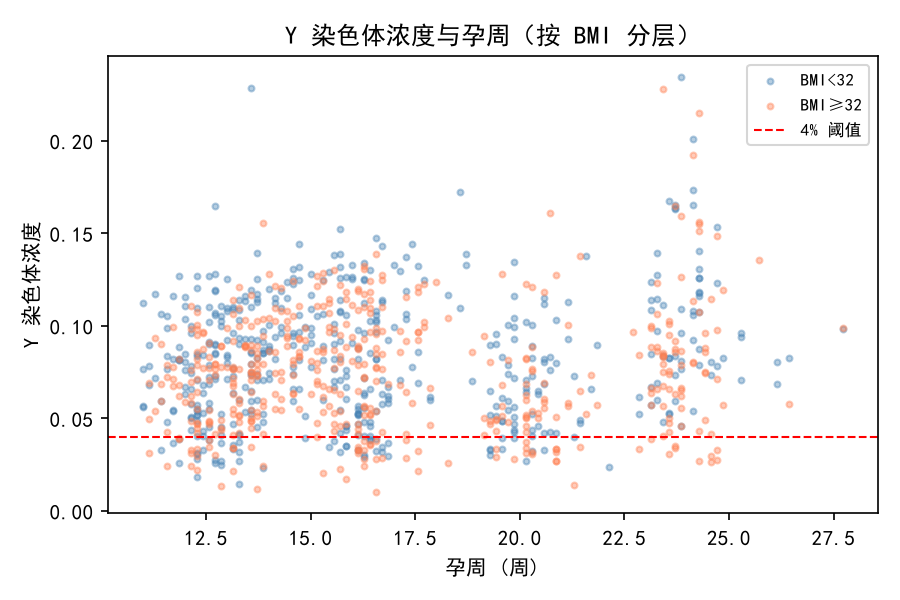
\includegraphics[width=0.75\textwidth]{figs/y_conc_by_week.png}
\caption{Y 染色体浓度与孕周（按 BMI 分层，红色虚线为 4\% 阈值）}
\label{fig:yconc}
\end{figure}

\begin{figure}[ht]
\centering
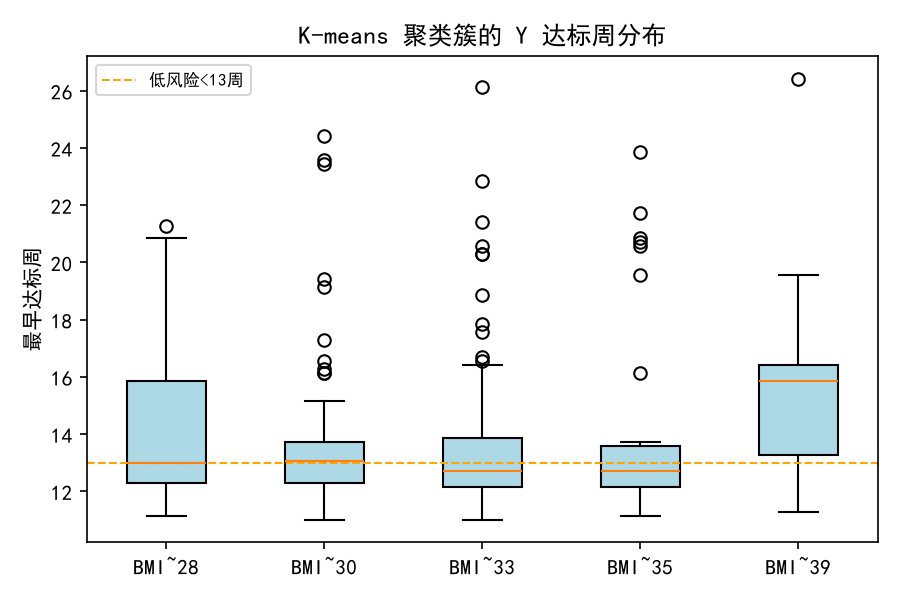
\includegraphics[width=0.75\textwidth]{figs/reach_week_by_cluster.png}
\caption{K-means 聚类簇的 Y 达标周分布（橙色虚线为 13 周低风险界）}
\label{fig:reach}
\end{figure}

\begin{figure}[ht]
\centering
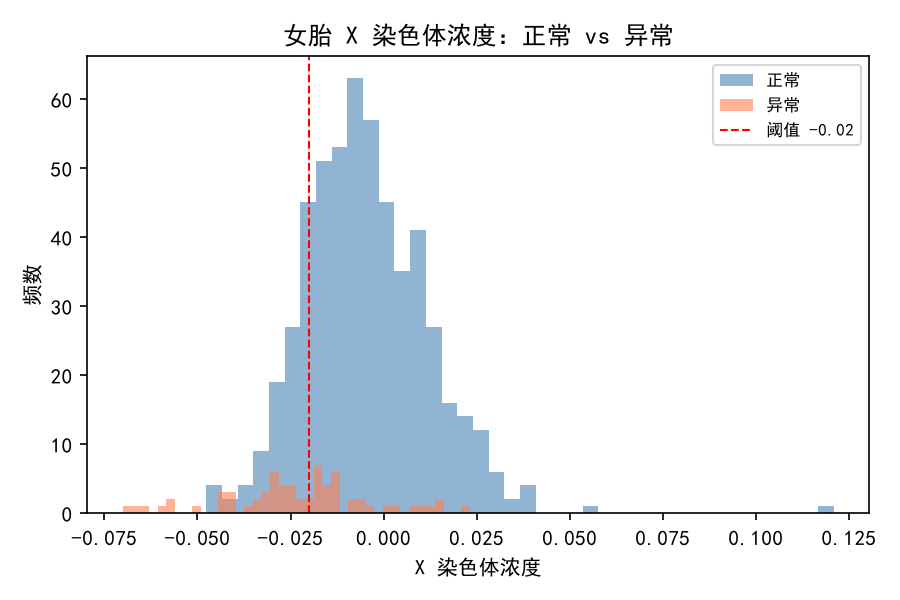
\includegraphics[width=0.75\textwidth]{figs/x_conc_by_anomaly.png}
\caption{女胎 X 染色体浓度：正常与异常分布（红色虚线为判定阈值 -0.02）}
\label{fig:xconc}
\end{figure}

\section{灵敏度分析}\label{sec:sensitivity}
Y 浓度测量误差 $\pm5\%$/$\pm10\%$ 对达标周判定影响小（3.1\%/3.5\%）；
聚类数 k=3/4/5 的分组结构稳定（中心漂移 $<1$）；女胎 X 浓度阈值在
$-0.03\sim-0.01$ 间灵敏度-特异度权衡清晰。

\section{模型评价与改进}\label{sec:evaluation}
\textbf{优点}：混合效应正确处理纵向重复测量（ICC=0.76 证明必要）；
K-means 数据驱动分组；女胎判定给出可操作阈值。
\textbf{不足}：高 BMI 极端组样本少（10 人），置信区间宽；女胎 AB 标记与
健康列不一致（检测疑似 vs 出生确认），未做标签敏感性分析。
\textbf{改进}：按异常类型分型建模（T18/T13 用 X 浓度、T21 需额外特征）；
引入出生健康结果做标签校正。

\bibliographystyle{plain}
\begin{thebibliography}{9}
\bibitem{deng2023} Deng C, et al. Maternal and fetal factors influencing fetal
fraction: A retrospective analysis of 153,306 pregnant women undergoing
noninvasive prenatal screening. Frontiers in Pediatrics, 2023.
\bibitem{fftrend2022} Non-intuitive trends of fetal fraction development
related to gestational age and fetal gender, and their practical implications
for non-invasive prenatal testing. ScienceDirect, 2022.
\bibitem{acmg2022} ACMG. Noninvasive prenatal screening (NIPS) for fetal
chromosome abnormalities in a general-risk population: evidence-based
clinical guideline. 2022.
\bibitem{kmnipt} NIPT Testing Timing Decision Algorithm Based on K-means
Clustering and Multi-Objective Risk Optimization. Semantic Scholar.
\end{thebibliography}

\appendix
\section{主要代码与结果}
求解脚本见 \texttt{c\_q1.py} 至 \texttt{c\_q4.py}，结果见
\texttt{q1\_result.md} 至 \texttt{q4\_result.md}。
\end{document}
